\documentclass[11pt,a4paper]{article}
\usepackage[margin=23mm]{geometry}
\usepackage[T1]{fontenc}
\usepackage{lmodern,microtype}
\usepackage{amsmath,amssymb,amsthm,bm}
\usepackage{booktabs,tabularx,array,longtable}
\usepackage{xcolor,hyperref,fancyhdr,enumitem}
\usepackage{tikz}
\usetikzlibrary{arrows.meta,positioning}
\definecolor{ink}{HTML}{172B46}
\definecolor{accent}{HTML}{157A83}
\definecolor{pale}{HTML}{EDF5F6}
\hypersetup{colorlinks=true,linkcolor=accent,urlcolor=accent,citecolor=accent,pdftitle={CSM: Mathematical Engineering of Persistent Regulation},pdfauthor={Woyengi Intelligence Labs}}
\setlength{\parindent}{0pt}
\setlength{\parskip}{5pt}
\setlist{nosep,leftmargin=1.5em}
\pagestyle{fancy}
\fancyhf{}
\fancyhead[L]{\small\color{ink}WOYENGI INTELLIGENCE LABS}
\fancyhead[R]{\small CSM-MATH-001}
\fancyfoot[L]{\small Mathematical specification and verification}
\fancyfoot[R]{\thepage}
\setlength{\headheight}{15pt}
\newtheorem{proposition}{Proposition}
\newcommand{\norm}[1]{\left\lVert#1\right\rVert}
\newcommand{\diag}{\operatorname{diag}}
\newcommand{\sigmoid}{\operatorname{sigmoid}}
\newcommand{\argmax}{\operatorname{argmax}}
\newcommand{\ind}{\mathbf{1}}
\newcommand{\R}{\mathbb{R}}
\newcolumntype{Y}{>{\raggedright\arraybackslash}X}

\begin{document}
\begin{center}
{\small\color{accent}RESEARCH ENGINEERING NOTE \quad 9 NOVEMBER 2026}\par
\vspace{5mm}
{\LARGE\bfseries\color{ink}CSM: Mathematical Engineering\\of Persistent Regulation}\par
\vspace{3mm}
{\large A controlled extension of the existing record-rewrite model}
\end{center}

\begin{abstract}
We specify a small, causal regulatory extension of the existing Compositional
State Model (CSM). A token-derived bank of exponential traces influences the
existing controller; record semantics, operations, links, readout and cursor
updates remain unchanged. The trace bank has a compact associative scan, but the
complete CSM retains its sequential record/controller dependency. We derive
boundedness, forgetting, routing-margin and conditional local-stability results;
identify precise limits of sigmoid overwriting and state-dependent gates; and
give parameter, arithmetic and memory accounting. A NumPy reference, exact
rational checks, smooth-subgraph gradient checks and Lean structural proofs
accompany this specification. No model was trained and no speed or quality gain
is established.
\end{abstract}

\section*{Engineering decision}
The initial candidate adds \textbf{12 regulatory coordinates} to the existing
CSM controller. Three groups of four coordinates use relaxation times
\(4,32,256\) observed tokens. The old record system is preserved so that a future
comparison can isolate regulation. These timescales are an illustrative frozen
engineering choice, not empirically selected optima.

The important results are:
\begin{itemize}
\item The added regulator and the existing bounded proposals preserve coordinate
bounds in exact arithmetic. This is not a global contraction or learning theorem.
\item Token-only regulator inputs allow a parallel affine scan. Feedback from
record updates would invalidate that precomputation claim.
\item Neutral regulatory injection recovers the baseline core trajectory.
\item A state-dependent write gate contributes a derivative term that must be
included in stability analysis.
\item A finite real sigmoid gain is below one; perfect decoded recall and exact
vector replacement are distinct properties.
\end{itemize}

\newpage
\tableofcontents
\newpage

\section{Baseline, provenance and scope}

The baseline is the record-rewrite computation documented in CSM-GRAPH-001 and
used in CSM-ADDRESS-002 [1,2]. The published recovery branch was read at commit
\texttt{3edc4f1} (the full identifier is recorded in provenance). Original artifacts and
checkpoints were not changed. The mathematical source was read in full before
this extension was designed.

The earlier ADDRESS-002 report establishes restricted supervised SET/recall
behavior; it does not establish language competence, general composition or
discovered addressing. This note is a mathematical engineering extension, not a
new measurement of those earlier checkpoints.

\textbf{Included:} a complete transition specification, an explicit regulator
clock, reset/padding rules, sufficient invariants, conditional local-sensitivity
analysis, forward and backward trace equations, dependency analysis, cost
accounting, an independently reviewed reference and structural formal checks.

\textbf{Deferred:} output-derived feedback, attractor/hysteresis mechanisms,
multiple operations per token, new read-only query semantics, exact replacement
actions, typed multi-relations, record allocation/reuse, and a new training
campaign. Each would change the experiment and needs its own contract.

The added bank is mathematically a diagonal state-space subsystem. Biological
motivation does not establish novelty. Related precedents include Clockwork
RNNs, Recurrent Independent Mechanisms and Neural Production Systems [3--5].

\section{State and temporal conventions}

Let \(S\) be the number of records, \(d\) the record width, \(O\) the number of
operation embeddings, \(h\) the transformation width and \(\nu\) the vocabulary
size. Before consuming token \(x_t\), write
\[
\mathcal S_t=(V_t,\ell_t,c_t,h^-_t,h_t,n_t,r_t).
\]
\begin{tabularx}{\linewidth}{@{}l l Y@{}}
\toprule
Component & Type & Meaning\\ \midrule
\(V_t\) & \(\{0,\ldots,S-1\}\to\R^d\) & Persistent record values.\\
\(\ell_t\) & \(\{0,\ldots,S-1\}\to\{0,\ldots,S-1\}\) & One outgoing link per record.\\
\(c_t\) & \(\{0,\ldots,S-1\}\) & Current record cursor.\\
\(h^-_t,h_t\) & \(\R^d\) each & Previous two input-token embeddings.\\
\(n_t\) & \(\mathbb N\) & Observed-token position.\\
\(r_t\) & \(\R^m\) & New regulatory traces; initially \(m=12\).\\
\bottomrule
\end{tabularx}

The initial values, histories and traces are zero; links are identity links and
cursor/position are zero. The initial state is explicit: there is no hidden
warm-up with future data. Model weights are fixed during a forward sequence.
After consuming \(x_t\), the logits predict \(x_{t+1}\). The next token may enter
the loss as a target, but cannot enter the state transition producing that loss.

\subsection{One clock and explicit boundaries}
The regulator advances once per \emph{observed token}, not per wall-clock second,
kernel invocation or future internal operation. Padding is an identity transition
with no output. A document reset occurs before a valid token and resets the
\emph{whole} original state as well as the regulator. Reset combined with padding
is invalid input. Processing chunks of one document carries all state across
chunks; a chunk boundary is not automatically a reset.

These choices affect the mathematical model. If an \(H\)-operation inner loop
updated a trace \(H\) times, its effective per-token decay would be \(\lambda^H\).
An extension with such a loop should freeze the token trace during the loop.

\section{Complete proposed forward equations}
All affine maps below include their original biases unless explicitly stated.
The hard categorical selector uses deterministic lowest-index tie breaking.
Temperature must be positive if a softmax precedes hard selection.

\subsection{Causal frontend and new regulatory path}
\begin{align}
e_t &= E(x_t),\\
f_t &= \tanh\!\left(F[h^-_t;h_t;e_t]\right),\\
s_t &= \tanh(Bf_t+b_r),\\
r_{t+1} &= \Lambda r_t+(I-\Lambda)s_t,\qquad
\Lambda=\diag(\lambda_1,\ldots,\lambda_m),\\
u_t &= \tanh\!\left(C[f_t;V_t(c_t)]+U_r r_{t+1}\right).
\end{align}
Here \(B\in\R^{m\times d}\), \(b_r\in\R^m\), and
\(U_r\in\R^{d\times m}\) are the only new learned arrays.
The decay values are fixed in the initial comparison.

Crucially, \(f_t\) uses previous \emph{input embeddings}, not previous controller
outputs. Given the token sequence and reset boundaries, every \(s_t\) can be
computed independently of the evolving record values. This is the exact sense
in which regulation is exogenous here. Perturbing the token history would also
perturb its features; independence is not claimed under that intervention.

\subsection{Unchanged reads, operation and proposal}
\begin{align}
i_t&=\argmax A_1u_t, & a_t&=V_t(i_t),\\
j_t^{\rm direct}&=\argmax A_2[u_t;a_t], &
j_t^{\rm link}&=\ell_t(i_t),\\
j_t&=\begin{cases}
j_t^{\rm link},&\text{use-link is selected and mode permits traversal},\\
j_t^{\rm direct},&\text{otherwise},
\end{cases}& b_t&=V_t(j_t),\\
k_t&=\argmax Ku_t,& o_t&=\Omega(k_t),\\
z_t&=\tanh\!\left(T_2\tanh\!\left(T_1[f_t;a_t;b_t;o_t]\right)\right).
\end{align}
One shared transformation is conditioned on the operation embedding. These
symbols do not imply that separate symbolic algorithms have been learned.
The second direct-address decision depends on the first retrieved value and
must not be scheduled as an independent controller-only head.

\subsection{Unchanged write, link, cursor and readout}
For ordinary rewrite mode, \(d_t=\argmax Du_t\). Ring-write mode uses
\(d_t=n_t\bmod S\). Let \(\epsilon_t\in\{0,1\}\) be the original hard
admission decision, \(\eta_t=\sigmoid(Gu_t)\), and
\(\alpha_t=\epsilon_t\eta_t\). Then
\begin{align}
w_t&=(1-\alpha_t)V_t(d_t)+\alpha_tz_t,\\
V_{t+1}&=V_t[d_t\mapsto w_t],\\
\ell_{t+1}&=\begin{cases}\ell_t[d_t\mapsto j_t],&\text{link edit selected},\\
\ell_t,&\text{otherwise},\end{cases}\\
c_{t+1}&=d_t,\quad h^-_{t+1}=h_t,\quad h_{t+1}=e_t,\quad n_{t+1}=n_t+1,\\
y_t&=Yw_t,\qquad p_\theta(x_{t+1}\mid x_{\le t})=\operatorname{softmax}(y_t).
\end{align}
The no-links mode disables traversal but retains the original link-update
computation. A rejected value edit preserves record values; it need not preserve
cursor, links, histories or traces. Calling it an identity of the entire state
would therefore be false.

\subsection{Baseline inclusion}
Setting \(U_r=0\) recovers the original controller and hence its original
core transition at every token. Induction gives equality of the core trajectory
and unchanged readout, assuming the same original weights and input features.
The added unused regulator can continue evolving, so equality of the entire
augmented state is not claimed. If initialized at zero, \(U_r\) also makes the
first-step task gradient to \(B,b_r\) zero; neutral initialization changes early
optimization and must be recorded rather than treated as costless training.

\section{Computational graph and dependency boundary}
\begin{center}
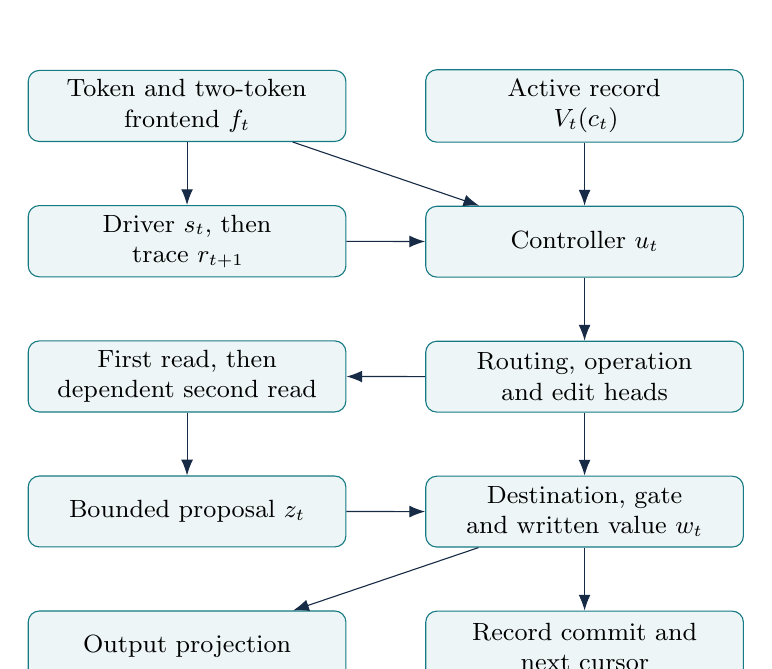
\begin{tikzpicture}[node distance=8mm and 10mm, every node/.style={font=\small},
 box/.style={draw=accent,rounded corners,fill=pale,align=center,text width=38mm,minimum height=9mm},
 arr/.style={-{Latex[length=2mm]},draw=ink}]
\node[box] (front) {Token and two-token\\frontend \(f_t\)};
\node[box,right=of front] (active) {Active record\\\(V_t(c_t)\)};
\node[box,below=of front] (driver) {Driver \(s_t\), then\\trace \(r_{t+1}\)};
\node[box,below=of active] (ctrl) {Controller \(u_t\)};
\node[box,below=of ctrl] (heads) {Routing, operation\\and edit heads};
\node[box,below=of driver] (read) {First read, then\\dependent second read};
\node[box,below=of read] (proposal) {Bounded proposal \(z_t\)};
\node[box,below=of heads] (write) {Destination, gate\\and written value \(w_t\)};
\node[box,below=of write] (commit) {Record commit and\\next cursor};
\node[box,below=of proposal] (output) {Output projection};
\draw[arr] (front)--(driver);
\draw[arr] (front)--(ctrl);
\draw[arr] (active)--(ctrl);
\draw[arr] (driver)--(ctrl);
\draw[arr] (ctrl)--(heads);
\draw[arr] (heads)--(read);
\draw[arr] (read)--(proposal);
\draw[arr] (heads)--(write);
\draw[arr] (proposal)--(write);
\draw[arr] (write)--(commit);
\draw[arr] (write)--(output);
\end{tikzpicture}
\end{center}
This is a dependency overview. Original link/history updates and individual
head branches are grouped for readability. The record store and previous trace
are inputs to their respective operations. Independent output and record-commit
branches both consume \(w_t\).

The recurrence \(V_{t+1}(c_{t+1})=w_t\) is unchanged. Thus
\(w_t\to u_{t+1}\to w_{t+1}\) remains a temporal dependency chain.
Parallelizing the regulatory branch does not remove this chain.

\section{Trace algebra, retention and scan}
Use \(\lambda_j=\exp(-1/\tau_j)\), where \(\tau_j\) is measured in observed
tokens. Its half-life is \(\tau_j\log 2\), not \(\tau_j\). For constant
\(\lambda_j\) without resets,
\begin{equation}
r_{t,j}=\lambda_j^t r_{0,j}
 +(1-\lambda_j)\sum_{k=0}^{t-1}\lambda_j^{t-1-k}s_{k,j}.
\end{equation}
The impulse kernel is \((1-\lambda_j)\lambda_j^n\). Longer retention also
means smaller initial input amplitude. With zero initialization and constant
input \(s_j=\mu_j\), the trace equals
\((1-\lambda_j^t)\mu_j\). This cold-start behavior is part of the model; it
is not an unbiased estimate of a stationary mean at every prefix length.

Represent one event as \(r' = a\odot r+b\). Ordinary tokens have
\(a=\lambda\), \(b=(1-\lambda)\odot s\); padding has \((a,b)=(1,0)\);
a reset followed by a valid token has \(a=0\), \(b=(1-\lambda)\odot s\).
Chronological composition is
\begin{equation}
(a_1,b_1)\diamond(a_2,b_2)
=(a_2\odot a_1,\ a_2\odot b_1+b_2).
\end{equation}
Both parenthesizations of three events give
\[
(a_3a_2a_1,\ a_3a_2b_1+a_3b_2+b_3),
\]
coordinatewise. Associativity therefore follows from associative multiplication,
associative addition and distributivity. The Lean theorem states these algebraic
laws explicitly as hypotheses; it does not silently add new logical axioms.

An ideal work-efficient scan uses \(O(Tm)\) arithmetic work and \(O(\log T)\)
parallel span for the already generated trace events. The serial checker
validates the scan algorithm's algebra; it is not a parallel speed benchmark.
Floating-point reassociation can change results, so exact-real or rational
equivalence must not be called bitwise FP32 equality.

\section{What is stable and what is only bounded}
\begin{proposition}[Coordinate invariance]
Assume finite real computations, initial values and traces in \([-1,1]\),
\(0\le\lambda_j\le1\), and \(0\le\alpha_t\le1\). Then all record-value
and trace coordinates remain in \([-1,1]\).
\end{proposition}
\begin{proof}
The driver and proposal use tanh and belong to the cube. Each trace update is
a coordinatewise convex combination. The selected record update is a convex
combination of the old record and its bounded proposal; all other records are
unchanged. Induct on tokens, including the zero reset and padding identity.
\end{proof}
This statement does not bound the unbounded natural-number position counter.
Nor does it prove that floating-point intermediates cannot overflow. The
reference rejects nonfinite inputs, but its finite tests are not a universal
IEEE refinement proof.

\begin{proposition}[Forgetting of regulatory initialization]
Within a reset-free segment of observed tokens, two traces exposed to identical
token features satisfy
\(\Delta r_t=\Lambda^t\Delta r_0\). If \(\rho=\max_j\lambda_j<1\), then
\(\norm{\Delta r_t}_\infty\le\rho^t\norm{\Delta r_0}_\infty\).
\end{proposition}
\begin{proof}
Subtract the two affine recurrences. The identical driving terms cancel.
Repeated substitution gives the stated identity and norm bound.
\end{proof}
A shared reset makes the initialization difference exactly zero; the norm
upper bound remains valid, but the reset-free equality must not be used across
that event. Padding does not advance the observed-token exponent.
If the inputs differ by at most \(\delta\) in a coordinate, their forced trace
difference is at most \((1-\lambda_j^t)\delta\), in addition to initialization
error. Feedback derived from model outputs generally prevents cancellation.

\subsection{The missing gate derivative}
On a fixed discrete-routing branch, let one record update be
\(G(w,r)=(1-\alpha(w,r))w+\alpha(w,r)z(w,r)\). Then
\begin{equation}
D_wG=(1-\alpha)I+\alpha D_wz+(z-w)(\nabla_w\alpha)^\top.
\end{equation}
The final term cannot be dropped. For the bounded scalar example
\[
G(v)=(1-\sigmoid(8v))v+\sigmoid(8v),
\]
the interval \([-1,1]\) is invariant, yet \(G'(0)=2.5\). Inputs \(0\) and
\(0.01\) become \(0.5\) and approximately \(0.524789446754\), expanding
their separation by \(2.4789446754\). This disproves a blanket nonexpansivity
claim; it does not show that a trained CSM diverges.

A separate bounded map \(G(v)=0.5v+0.5\tanh(3v)\) has a fixed point at zero
with derivative two. Thus boundedness also does not imply stability of every
equilibrium. Both counterexamples remain inside the bounded-proposal family.

\subsection{A valid sufficient local condition}
Hold discrete routes and other read records fixed. Suppose throughout a convex
neighborhood that
\[
\alpha\ge\alpha_{\min}>0,\quad
\norm{D_wz}\le L_z<1,\quad
\norm{\nabla_w\alpha}_*\le L_\alpha,\quad
\norm{z-w}\le D.
\]
Then
\begin{equation}
\norm{D_wG}\le q_w:=1-\alpha_{\min}(1-L_z)+DL_\alpha.
\end{equation}
The condition \(q_w<1\) suffices for local contraction of this active-record
map at fixed regulator. For a sigmoid gate on an admitted branch,
\(L_\alpha\le L_g/4\) if the gate logit has gradient norm at most \(L_g\).
These quantities have not been certified for trained model weights.

If additionally \(\norm{D_rG}\le K_r\), the active record and exogenous trace
obey
\[
\norm{\Delta w^+}\le q_w\norm{\Delta w}+K_r\rho\norm{\Delta r},\qquad
\norm{\Delta r^+}\le\rho\norm{\Delta r}.
\]
For any \(Q\) with \(\max(q_w,\rho)<Q<1\), choose
\(c>0\) with \(c\ge K_r\rho/(Q-\rho)\). The weighted norm
\(\norm{\Delta w}+c\norm{\Delta r}\) then contracts by at most \(Q\).
This result treats other read records as identical external inputs.

The full bank does not inherit strict contraction. On a fixed routing branch,
untouched continuous records retain identity coordinates. Reordering coordinates
gives an identity block and eigenvalue one whenever an untouched record remains.
Persistent exact memory is compatible with this absence of global forgetting.

\subsection{Hard-route margins}
Let \(\xi\) denote the complete input to a routing-logit map, including any
relevant record values. If every routing logit is locally \(L\)-Lipschitz and the winning logit's margin
over every competitor is \(\gamma>0\), then
\begin{equation}
\norm{\Delta\xi}<\frac{\gamma}{2L}
\end{equation}
preserves the route, for \(L>0\). Each of the two logits changes by at most
\(L\norm{\Delta\xi}\), so their difference remains positive. A bound on the
driver \(s_t\) alone would not constrain record-induced route changes. This is a
one-decision guarantee. Every relevant hard decision must keep its margin
before a smooth fixed-branch Jacobian argument can apply across a rollout.

\section{Write semantics and safe composition}
For fixed target \(z\), one admitted write satisfies
\begin{equation}
w^+-z=(1-\alpha)(w-z).
\end{equation}
A finite real sigmoid gain has \(\alpha<1\); it leaves a nonzero vector residual
when \(w\ne z\). Repeated writes give
\(e_N=\prod_{k=0}^{N-1}(1-\alpha_k)e_0\). With
\(\alpha_k\ge\alpha_{\min}>0\), error decreases geometrically. With
\(\alpha=0.5\), reducing error one below \(10^{-6}\) takes 20 writes.
Floating-point sigmoid may round to one, but rounding is not an exact-real
replacement contract.

Decoded classification can nevertheless be exactly correct. Suppose every
readout logit is \(L\)-Lipschitz and the intended class at \(z\) has margin
\(\gamma\). A sufficient condition for the same decoded class after writing is
\[
(1-\alpha)\norm{w-z}<\gamma/(2L).
\]
Thus perfect discrete recall does not establish exact vector copying. A later
exact-COPY experiment must either permit hard replacement or state a semantic
decoding/error contract. Changing this now would confound the regulator ablation.

\subsection{Dependence-aware parallel edits}
For complete read/write footprints, sufficient conditions for two recomputed
transactions to commute are
\[
W_A\cap W_B=\varnothing,\quad W_A\cap R_B=\varnothing,\quad W_B\cap R_A=\varnothing.
\]
Footprints include routing inputs, guards, cursor and regulatory dependencies.
Different destinations alone are insufficient. Starting from \((A,B)=(0,1)\),
the two updates \(A\leftarrow(A+B)/2\), \(B\leftarrow(B+A)/2\) produce
\((0.5,0.75)\) in one order and \((0.25,0.5)\) in the other. Simultaneous
snapshot evaluation gives \((0.5,0.5)\).

The new Lean theorem proves the narrower, explicit contract: \emph{already
computed proposals from one frozen snapshot} commute when committed to distinct
slots. It does not prove equality to proposals recomputed after earlier edits,
or commutation of complete CSM token steps.

\section{Training derivatives and information contract}
Ordinary task training remains causal next-token or answer prediction. Optional
controller labels enter additional losses; they do not become forward inputs.
All conditions must use model-produced state at inference. Supplying correct
addresses during evaluation is a separately labeled capacity diagnostic.

For the smooth trace/controller path, write \(s_t=\tanh(Bf_t+b_r)\),
\(r_t=\lambda\odot r_{t-1}+(1-\lambda)\odot s_t\), and
\(u_t=\tanh(b_t^{\rm core}+U_rr_t)\), where
\(b_t^{\rm core}=C[f_t;V_t(c_t)]\) is the original controller's affine
preactivation, including its bias. If \(\bar u_t\) is the incoming adjoint,
\begin{align}
\bar q_t&=\bar u_t\odot(1-u_t^2),\\
\bar r_t&=U_r^\top\bar q_t+\lambda\odot\bar r_{t+1},\\
\bar a_t&=(1-s_t^2)\odot(1-\lambda)\odot\bar r_t,\\
\nabla_B L&=\sum_t\bar a_t f_t^\top,\quad
\nabla_{b_r}L=\sum_t\bar a_t,\quad
\nabla_{U_r}L=\sum_t\bar q_t r_t^\top.
\end{align}
Here indices are shifted to name the trace after its token. In a full reverse
graph, \(\bar u_t\) includes all downstream contributions through record
computation; the equations do not omit those paths. Across a reset, trace
backward carry is zero. Across padding it is unchanged.

The supplied checker tests a squared-error loss on this smooth subgraph with
fixed frontend features and a simplified, frozen base input \(b_t^{\rm core}=Af_t\).
It validates \(B,b_r,U_r\) and the initial trace against
central finite differences. It does not validate the entire CSM backward pass.

The baseline uses hard categorical forward choices with a supplied softmax
straight-through backward rule [1,6]. That rule is not the ordinary derivative
of argmax. The new smooth-path check cannot establish that this estimator is
unbiased, that sparse forward routing makes its backward sparse, or that it
learns the intended actions. Those remain explicit training obligations.

\section{Parameter, work and memory accounting}
With fixed decays, the added driver and controller projection require
\begin{equation}
\Delta P=md+m+dm=2dm+m,\qquad
\Delta W_{\rm MAC}=2dm,\qquad \Delta M_{\rm FP32}=4m\ \text{bytes}.
\end{equation}
MACs count only nominal dense dot-product terms; biases, tanh, trace recurrence,
selection, allocation, bandwidth, backward and optimizer work are excluded.
These formulas are not measured latency or a complete FLOP count.

The original source formulas are
\begin{align*}
P_0&=2\nu d+\nu+5d^2+4Sd+3S+2Od+O+5dh+h+10d+7,\\
W_0&=5d^2+8Sd+2Od+5dh+d\nu+S^2+7d,\\
M_0/4&=Sd+S^2+S+2d.
\end{align*}
For \(S=8,d=32,O=4,h=64,\nu=19,m=12\):
\begin{center}
\begin{tabular}{lrrr}
\toprule
Quantity & Baseline & Candidate & Addition\\ \midrule
Allocated learned parameters & 18,294 & 19,074 & 780\\
Nominal dense MAC terms/token & 18,560 & 19,328 & 768\\
Retained FP32 tensor bytes/stream & 1,568 & 1,616 & 48\\
\bottomrule
\end{tabular}
\end{center}
The new reference independently instantiates the reported parameter count.
The cache and MAC accounting intentionally describes the original dense-source
convention. The NumPy reference uses indexed integer links and float64, so these
are not its actual allocated bytes or runtime operations. The dense cache count
excludes position integer, parameters, outputs, training activations and allocator
overhead. Bounded inference state does not imply constant training memory.

\section{Controlled comparison to run next}
\begin{tabularx}{\linewidth}{@{}l Y l@{}}
\toprule
Condition & Decay configuration & Added arrays\\ \midrule
Original & No regulatory path & None\\
Immediate & All \(\lambda_j=0\) & \(B,b_r,U_r\)\\
Single timescale & All \(\tau_j=32\) & Same shapes\\
Multiple timescales & Four channels at each \(\tau=4,32,256\) & Same shapes\\
\bottomrule
\end{tabularx}
Immediate, single and multiple conditions have identical parameters and feature
dimensions. Single and multiple have equal persistent-state capacity. The
immediate implementation can omit carried traces in deployment; retaining the
same reference container does not make that information necessary. The original
baseline is smaller and must be identified as such.

The comparison must hold data, answer/controller supervision, optimizer,
initialization policy and update budget constant within each condition group.
The earlier supervised SET task is already at a reported ceiling; it is a
preservation check, not a useful sole measure of improvement. New changing-history
conditions must specify the decision target and eliminate shortcuts. Evaluate
delayed commitment, irrelevant writes, valid corrections, missing queries and
regime changes separately. Keep oracle-control diagnostics separate.

Reset/swap interventions on the traces test causal use of the added state.
Per-seed results and collapse rates are required. After elementary control is
reliable, test new operation combinations and longer chains, then held-out
language. With the user's inference priority, every new projection and operation
must enter end-to-end latency measurement; algebraic MAC savings alone cannot
qualify an efficiency result.

\section{Verification performed and remaining boundary}
\begin{tabularx}{\linewidth}{@{}p{33mm}Y@{}}
\toprule
Evidence & Recorded result and scope\\ \midrule
Reference execution & Zero-injection baseline equality, prefix causality,
nonmutation, selected-write frames, bounds, reset, padding and independent
streams passed on deterministic fixtures in float64. No archived checkpoint
or original PyTorch-runtime parity is claimed.\\
Exact trace algebra & Finite Fraction checks passed for affine associativity,
closed form, serial/tree-scan equality, reset, padding and chunk continuation.
Candidate exponentials are represented by the exact fractions of their
binary64 approximations.\\
Smooth gradients & 64 coordinate comparisons across four boundary conditions
passed; maximum absolute discrepancy \(4.038687023699694\times10^{-10}\).
This is restricted to the smooth regulator/controller subgraph.\\
Stability review & 14 deterministic checks passed, including gate-Jacobian and
bounded-instability counterexamples, a constructed sufficient-contraction
case, route margins and write-order conflicts.\\
Lean structural proofs & 23 theorem declarations compile with Lean 4.19.0,
\texttt{--trust=0}. Parent verification performs a fresh build, declared-theorem
axiom audit and deliberately false proof controls; see
\texttt{verification/lean.json}.\\
\bottomrule
\end{tabularx}

Lean covers pure-transition structural statements and affine composition under
explicit algebra-law hypotheses. The real-valued boundedness and local-stability
arguments in this document have been independently reviewed and numerically
corroborated; they are not newly machine-checked real-analysis proofs. The
formal abstraction's input is a prepared causal token feature, so exogeneity
requires identical feature histories and reset boundaries. Output equality
additionally requires the unchanged readout on identical core state/features.

The official Lean executable encountered the same application-path discovery
failure documented by the earlier project. The existing disclosed C launcher
supplies the known executable path and invokes the unchanged official
\texttt{lean\_main} shared library. It changes no kernel, elaborator, proof
operation, permissions or sandbox setting. Source and toolchain hashes are
recorded. This is an adapted-launcher verification, not a second independent
proof-kernel implementation.

No mathematical statement here proves a semantic role binding, useful operation
specialization, correct factual belief, learning convergence, neural-model
quality, biological fidelity, architectural novelty, or wall-clock speedup.
The next empirical decision is whether the added regulator improves control
enough to justify its inference cost.

\section*{Reproduction}
From the delivered source directory:
\begin{verbatim}
python3 verify_reference.py
python3 trace_algebra.py > verification/trace_algebra.json
python3 verify_stability.py
python3 verify_trace_gradients.py
python3 verify_lean.py --lean /path/to/lean
pdflatex -interaction=nonstopmode -halt-on-error specification.tex
\end{verbatim}
The optional launcher flags and full frozen source hashes are in the accompanying
verification files. Use a fresh copy or retain old receipts before rerunning;
do not overwrite evidence being used for comparison. The Python reference needs
NumPy; the exact trace checker uses only Python's standard library. Lean uses
\texttt{Std} without Mathlib. PDF generation uses standard LaTeX packages.

\section*{References}
\begin{enumerate}[label={[\arabic*]}]
\item Woyengi Intelligence Labs. \emph{CSM-GRAPH-001: Mathematical model,
parallel execution, and Lean verification}. 9 November 2026.
\href{https://github.com/FPC-effortless/cdl-attention-experiment/blob/3edc4f1a541a3221390e4c0a21fe0c12004f1ca5/artifacts/csm-original-scope-reconstructed-20261109/CSM-GRAPH-001-verified-project.zip}{Published verified-project archive}.
\item Woyengi Intelligence Labs. \emph{CSM-ADDRESS-002: controller supervision
repairs SET and recall in a bounded task}. 9 November 2026.
\href{https://github.com/FPC-effortless/cdl-attention-experiment/blob/3edc4f1a541a3221390e4c0a21fe0c12004f1ca5/artifacts/csm-address-002-recovered-20261109/CSM-ADDRESS-002-results.md}{Published report at the inspected commit}.
\item Koutnik et al. \emph{A Clockwork RNN}. ICML, 2014.
\url{https://proceedings.mlr.press/v32/koutnik14.html}.
\item Goyal et al. \emph{Recurrent Independent Mechanisms}.
arXiv:1909.10893, 2019; revised 2020.
\url{https://arxiv.org/abs/1909.10893}.
\item Didolkar et al. \emph{Neural Production Systems}. NeurIPS, 2021.
\url{https://research.google/pubs/neural-production-systems/}.
\item Bengio, L\'eonard and Courville. \emph{Estimating or Propagating Gradients
Through Stochastic Neurons for Conditional Computation}. 2013.
\url{https://arxiv.org/abs/1308.3432}.
\end{enumerate}
\end{document}
